%-----------------
% Header
%-----------------
\documentclass[
a4paper,                % Papierformat A4
12pt,										% Schriftgr��e 12pt
oneside, 								% Zweiseitiges Layout [oneside]
titlepage,              % Titleseite verwenden
headsepline,            % Trennlinie zum Seitenkopf Bereich headings
bibliography=totoc,     % Das Literaturverzeichnis in den TOC
listof=totoc, 					% alle Listen in das Inhaltsverzeichnis
cleardoublepage=plain
]{scrbook}

\bibliographystyle{alphadin}

%-----------------
% Packages
%-----------------
\usepackage[ngerman]{babel}
\usepackage{textcomp}
\usepackage[T1]{fontenc}
\usepackage[latin1]{inputenc}
\usepackage{lmodern}
\usepackage{lscape}
\usepackage{rotating}
\usepackage{tocbasic}
\usepackage{color}
%\usepackage{palatino}
%\usepackage{mathpazo}
%\usepackage{courier}
% left = innen, right = au�en
\usepackage[a4paper, left=4cm, right=3cm, top=4cm, bottom=4cm]{geometry} 

\usepackage{graphicx, amsmath, longtable, booktabs, color, listings, makeidx, pdfpages, subfigure, amsfonts}
\usepackage{float}
\usepackage[pdftex,
	hyperindex=true,
	plainpages=false,
	hypertexnames=true,
	bookmarks=true,
	bookmarksnumbered=true,
	pdfhighlight=/O,
	linkcolor=black,
	citecolor=black,
	filecolor=black,
	menucolor=black,
	urlcolor=black,
	colorlinks=true,
	pdftitle={Ruby on Rails},
	pdfauthor={Alexander Miller},
	pdfsubject={Dokumentation: Ruby on Rails},
	pdfstartpage=1]{hyperref}
	
\hyphenation
{
	soft-ware-m�-�i-gen
	kryp-to-gra-phi-schen
	kryp-to-gra-phi-scher
	Ein-weg
	Hash-funk-ti-o-nen
	Pro-to-kol-le
}
	
% Formatierung f�r Code-Listings setzen:
\lstset{basicstyle=\scriptsize\ttfamily,
		keywordstyle=\bfseries\color[rgb]{0.07, 0.21, 0.45},
		keywordstyle=[2]\color[rgb]{0.3, 0.4, 0.5},
		commentstyle={\color[gray]{0.5}\textit},
		stringstyle={\textit},
		xleftmargin=0.5cm, xrightmargin=0cm, framerule=1pt,
		showstringspaces=false, breaklines=true, breakatwhitespace=true,
		numbers=left, numberstyle=\tiny, stepnumber=1, numbersep=0.2cm,
		frame=lines,
		aboveskip=\bigskipamount, belowskip=\bigskipamount,
		framexleftmargin=0.5cm,
		tabsize=4,
		escapeinside={<ref>}{</ref>}}
%--------------------------------------
%   Metainformation
%--------------------------------------
\newcommand{\art}{Angewandte Informatik}
\newcommand{\titel}{Konzeption und Entwicklung einer CD-Tauschb�rse mit \\Ruby on Rails}
\newcommand{\untertitel}{\empty}
\newcommand{\autor}{Christian Bunk \\ Alexander Miller \\ Christian Sandvo� \\ Antonia Ziegler}
\newcommand{\hochschule}{Hochschule f�r Technik und Wirtschaft Berlin}
\newcommand{\fachgebiet}{Angewandte Informatik}
\newcommand{\erstgutachter}{Prof. Dr. Albrecht Fortenbacher}
\newcommand{\datum}{Abgabedatum: 08.01.2012} % durch Abgabedatum zu ersetzen
\newcommand{\ort}{Berlin}


	
%--------------------------------------
%   Dokumentenbeginn
%--------------------------------------
\begin{document}

%--------------------------------------
%   Titelseite
%--------------------------------------
\begin{titlepage}
	\pdfbookmark[-1]{\titel}{Marke}
	% Titelblattkopf
	\titlehead{
		\begin{flushright}
			
\includegraphics[width=0.45\textwidth]{images/HTW_Logo_rgb.jpg}
		\end{flushright}
	}
	\subject{\art \\ Systementwicklung und Frameworks\\ } % Art der Arbeit
	\title{\titel}% Titel der Arbeit
	\subtitle{\untertitel}% ggf. Untertitel
	\author{\autor}% Verfasser
	\date{\datum}% Datum
	\publishers{\erstgutachter}% Betreuer
	\maketitle %erzeugt die Titelseite
\end{titlepage}

%--------------------------------------
%   Seitennummerierung
%--------------------------------------
\pagenumbering{Roman}

%--------------------------------------
%   Abstract und Kurzfassung
%--------------------------------------
%Inhaltsverzeichnis:
\tableofcontents
%\addcontentsline{toc}{chapter}{Inhaltsverzeichnis}
%Abbildungsverzeichnis:
%\listoffigures
%\addcontentsline{toc}{chapter}{Abbildungsverzeichnis}
%Tabellenverzeichnis:
%\listoftables
%\addcontentsline{toc}{chapter}{Tabellenverzeichnis}
%Listingverzeichnis:
%\lstlistoflistings
%\addcontentsline{toc}{chapter}{Listingsverzeichnis}




\pagenumbering{arabic}

\chapter{Einleitung}
\label{sec:Einleitung}

In der Softwaretechnik wird unter dem Begriff Framework ein Ordnungsrahmen verstanden, innerhalb dessen die Entwickler eine Anwendung erstellen. Das Ziel ist die Definition einer einheitlichen Struktur mittels komponentenbasierten Entwicklungsans�tzen sowie die Vereinfachung der Entwicklung durch die Verwendung von zur Verf�gung stehenden Frameworks-Bestandteilen. Im Laufe der Lehrveranstaltung ''Systementwicklung und Frameworks'' wurden die Prinzipien der unterschiedlichen Frameworks wie zum Beispiel EJB und .NET vorgestellt und diskutiert. Als Pr�fungsleistung muss ein Projekt erfolgreich realisiert werden, wobei jede Gruppe von vier bis f�nf Personen die Anwendung mit einem ausgew�hlten Framework entwickeln m�ssen. 

In der vorliegenden Ausarbeitung handelt es sich um eine Dokumentation zum Projekt, wobei eine CD-Tauschb�rse konzipiert und implementiert wurde. Wie in der Aufgabenstellung bzw. im Pflichtenheft definiert (Anhang A.1) wurde eine Rich-Applikation (RIA) modelliert und entwickelt, wobei die meisten Funktionalit�ten nicht von Hand, sondern durch die Verwendung von Framework-Komponenten realisiert wurden. Die Gruppe besteht aus vier Personen (Christian Bunk, Alexander Miller, Christian Sandvo�, Antonia Ziegler) und entwickelt das Projekt mit dem Framework ''Ruby on Rails''. 

Ruby on Rails ist ein Framework f�r Webapplikationen, welches in der Programmiersprache Ruby entwickelt wurde. Model-View-Controller (MVC) Architektur erm�glicht eine Isolation der Businesslogik von der graphischen Benutzeroberfl�che und gew�hrleistet das ''don't repeat yourself'' (DRY) Prinzip. 

Der SourceCode wird mit Git (https://github.com/christianb/SE-FW) verwalten. Hierzu wird die online Plattform GitHub als zentrales Repository verwendet, die sowohl die aktuellen Aufgaben (Issues) als auch die Meilensteine verwaltet. Um eine Arbeitsgrundlage zu erschaffen, haben alle Gruppenmitglieder sich das grundlegende Wissen �ber das ausgew�hlte Framework angeeignet. Wie die geforderten Funktionalit�ten im Einzelnen implementiert sind, kann den folgenden Kapiteln entnommen werden. An dieser Stelle muss noch erg�nzt werden, dass alle gestellten Anforderungen erf�llt wurden.

\chapter{Ruby-on-Rails Framework}
\label{sec:Ruby on Rails Framework}

Ruby On Rails (Rails) ist ein Web-Framework welches auf der Programmiersprache Ruby basiert. Ruby ist eine Objektorientierte Programmiersprache. Anweisungen werden nicht durch ein Semikolon abgeschlossen sondern durch einen Zeilenumbruch. Jede Rails Anwendung hat eine feste Ordnerstruktur und verfolgt das Prinzip ''Convention Over Configuration''. Was bedeutet das der Konfigurationsaufwand durch einhalten von Konventionen so gering wie m�glich gehalten werden soll. Zus�tzlich zu allen erstellten Controllern wird auch ein so genannter Application-Controller erstellt. Alle weiteren Controller sind Unterklassen von diesem und erben daher auch alle Methoden die darin deklariert wurden. Im n�chsten Abschnitt sind die wichtigsten Konventionen n�her erl�utert.
\section{Rails-Konventionen}
\label{KOnventionen}
Wie oben erw�hnt verfolgt Rails das Konzept ''Convention Over Configuration''. Darunter fallen z.B. die Namenskonventionen welche besagen, dass die Namen der Controller m�glichst im Plural benannt werden und Models im Singular. Des Weiteren wird die Schreibweise von Variablen- und Klassennamen geregelt. Durch diese Konventionen weiss Rails welcher Controller zu welchen Model geh�rt, sowie welche Views zu einem Controller. Dadurch entf�llt die explizite Zuweisung zwischen den einzelnen Komponenten. Die Methoden im Controller werden Actions genannt. Zu jeder Action gibt es meist eine View welches �quivalent zur Bezeichnung der Action benannt ist. Sobald einen View und eine Action den gleichen Namen haben, wird beim Aufruf dieser automatisch die entsprechende View geladen.
\section{Model-View-Controller (MVC)}
\label{MVC}
Das Rails-Framework ist nach dem Model-View-Controller Konzept aufgebaut. Dabei dient das Model zur Kommunikation mit der Datenbank. Au�erdem sorgt es durch Validierung daf�r, dass Daten im korrekten Format in die Datenbank geschrieben werden. Die Views sind die HTML-Seiten, welche dem Nutzer angezeigt werden. Sie dienen zur Anzeige der Daten aus der Datenbank oder dem Erfassen von Nutzereingaben mit Hilfe von Formularen bzw. Eingabefeldern. Der Controller ist der Vermittler zwischen der View und dem Model. Er empf�ngt Daten von der View und sendet sie an das Model weiter. Umgekehrt werden Daten vom Model �ber den Controller der View zur Verf�gung gestellt.
\section{Don't Repeat Yourself (DRY)}
\label{DRY}
DRY beschreibt das ''Don't Repeat Yourself'' Konzept. Dies bedeutet das so wenig wie m�glich Code dupliziert wird. Zur Einhaltung dessen gibt es in Rails einigen Vorkehrungen. Als erstes w�ren da die Helper-Methoden zu nennen. Dies sind Methoden welche oft dazu genutzt werden, h�ufig genutzten Code durch Schl�sselw�rter zu ersetzen. Die Helper-Methoden werden meist in den Views verwendet um dort HTML-Code zu generieren. Ein oft verwendeter Helper ist beispielsweise ''link-to'', welcher den aus HTML bekannten Link-Tag generiert.

Ein weiterer Punkt ist die Definition des Seitenlayouts. Das Layout legt die Darstellung bzw. das Aussehen der HTML-Seiten fest. Dabei kann ein globales, f�r alle Seiten g�ltiges Layout definiert werden oder auch Layout-Vorlagen f�r spezielle Seiten definiert werden. Das Layout welches mit ''application.html.erb'' benannt wird, ist f�r alle Seiten g�ltig. Falls ein anderes Layout verwendet werden soll, muss diese explizit eingebunden werden. Ansonsten wird immer das in der Datei ''application.html.erb'' definierte genutzt. Das gleiche gilt auch f�r den Application-Controller. Hier definierte Methoden sind in allen anderen Controllern verf�gbar und m�ssen dadurch nicht in jedem Controller separat implementiert werden.

Seit der Version 3.1 von Rails, wird standardm��ig jQuery als Javascript Framework verwendet. Auch hier gibt es eine globale Datei (application.js) auf die aus allen Views zugegriffen werden kann. Javascript Code wird in der Regel nicht in den Views eingef�gt, sondern es wird auf die zu ver�ndernden HTML Elemente durch dessen IDs oder Klassen zugegriffen. Dies dient den Prinzip des Unobtrusive (unaufdringlich) Javascript und erh�ht die Lesbarkeit des Codes der Views. Eine weitere Neuerung der Version 3.1, ist die Asset-Pipeline. Darin werden die CSS und JavaScript Dateien gespeichert. Diese werden dann, vor Auslieferung an den Browser komprimiert, um die zu �bertragene Datenmenge zu verringern und dadurch die Zugriffszeit zu erh�hen.

\section{Object-Relation-Mapper (ORM)}
\label{ORM}
Um bei Rails Objekte in einer Datenbank zu speichern, kommt der Object-Relation-Mapper ActiveRecord zum Einsatz. Dabei werden die Tabellen als Klasse gesehen, die Zeilen als Objekt und die Spalten sind die Objekt-Attribute. Durch den ORM m�ssen keine SQL-Statements mehr geschrieben werden, sondern f�r den Zugriff auf die Datenbank werden Methoden genutzt. Beim erstellen einer Tabelle werden von Rails automatisch Methoden generiert. Eine Klasse hat unter andren die Methoden ''new'' und ''find''. Diese dienen zum erstellen oder finden eines Objekts. Das Objekt besitzt die Methoden ''save'', ''update'' und ''delete''. Diese werden zum Speichern, Aktualisieren und L�schen genutzt.

\chapter{Anwendung}
\label{sec:Anwendung}

\section{Projektmanagement}
\label{sec:Projektmanagement}

Eine der wichtigsten Aufgaben bei der Realisierung eines informationstechnischen Projektes ist das Projektmanagement. Es ist �u�erst wichtig eine genaue Planung sowie die Konzeption durchzuf�hren, damit alle Anforderungen, Termine und der Kostenrahmen eingehalten werden. In den n�chsten Kapiteln wird es beschrieben wie das Projektmanagement erfolgte, wobei intensiv auf die Meilensteinplanung sowie die Versionsverwaltung und Deployment eingegangen wird.

\subsection{Meilensteinplanung}
\label{Meilensteinplanung}

Um das Zeitmanagement zu organisieren, wurde die Meilensteinplanung durchgef�hrt. Es wurde vereinbart, dass bei der Entwicklung der meisten Funktionalit�ten immer zwei Gruppenmitglieder beteiligt sein m�ssen, um bei krankheitsbedingten Ausf�llen eines Gruppenmitglieds die Entwicklung fortsetzen zu k�nnen. 

\begin{figure}[ht]
\centering
		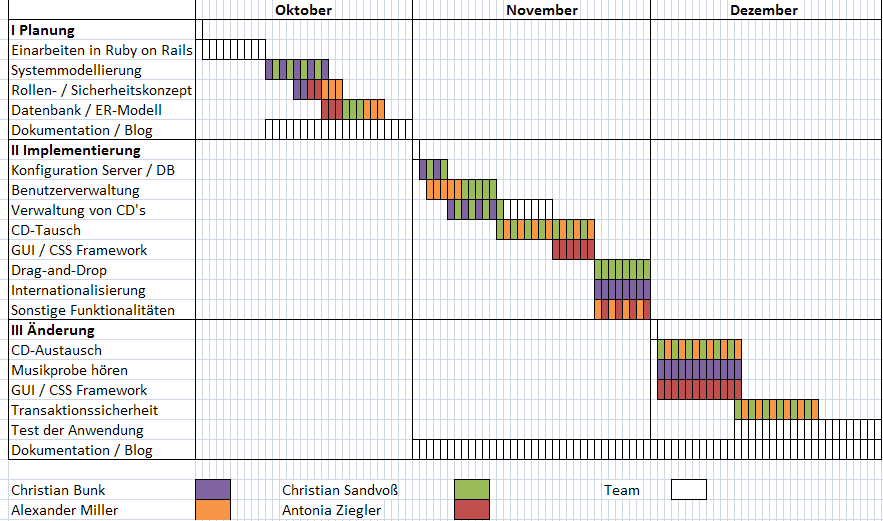
\includegraphics[height=7.2cm]{images/pm.png}
	\caption[Meilensteinplanung]{Meilensteinplanung}
	\label{fig:Meilensteinplanung}
\end{figure}

Dar�ber hinaus wurde es bestrebt, die Konzeption sowie die Systemmodellierung als Gruppenarbeit durchzuf�hren. F�r diese Zwecke wurden w�chentliche Termine (dienstags 12:00-14:00 und donnerstags 11:15 - 12:30) vereinbart. An diesen Terminen wurden in Rahmen einer Gruppenarbeit sowohl die aufgetretenen Schwierigkeiten gel�st, die w�chentliche Pr�sentation vorbereitet als auch der weitere Projektverlauf diskutiert.

\subsection{Versionsverwaltung von Quellcode}
\label{Versionsverwaltung von Quellcode}

F�r die Quellcode-Verwaltung wurde ein GitHub-Repository verwendet. Dabei wurde an das Branching-Modell orientiert, die in ( http://nvie.com/posts/a-successful-git-branching-model/) vorgestellt wird. 

\begin{figure}[ht]
\centering
		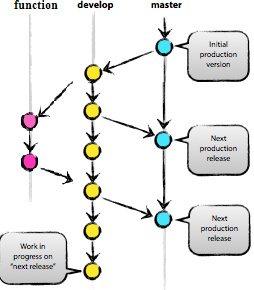
\includegraphics[height=7cm]{images/verlauf.png}
	\caption[Git - Function, Develop und Master Branches]{Git - Function, Develop und Master Branches}
	\label{fig:git1}
\end{figure}

Dabei wird folgende Strategie verfolgt: Als erstes werden zwei Branches angelegt \textit{develop} und \textit{master}. Die eigentliche Entwicklung geschieht auf dem \textit{develop} Branch und lediglich die Zwischenversionen, die eine neue und vor allem fehlerfreie Implementierung eine zus�tzlichen Funktionalit�t beinhalten, werden auf den \textit{master} Branch gelegt. Durch das Erstellen von weiteren Branches f�r die jeweilige Funktionalit�t kann weiterer Komfort bei der Entwicklung erreicht werden. Jede zus�tzliche Funktionalit�t wird dabei separat entwickelt, so dass eine Aufteilung der Aufgaben sowie die anschlie�ende Zusammenf�hrung der Quelltexte ohne Einschr�nkungen und Probleme erfolgen k�nnen. Wenn eine Funktion fertig gestellt worden ist, wird diese ins \textit{develop} Branch kopiert. Falls mehrere Funktionalit�ten im \textit{develop} Branch getestet und die identifizierten Fehler behoben wurden, wird die Anwendung ins \textit{master} Branch gemergt. Bei der Einhaltung des vorgestellten Models sieht die Quellcode-Verwaltung wie folgt aus:

\begin{figure}[ht]
\centering
		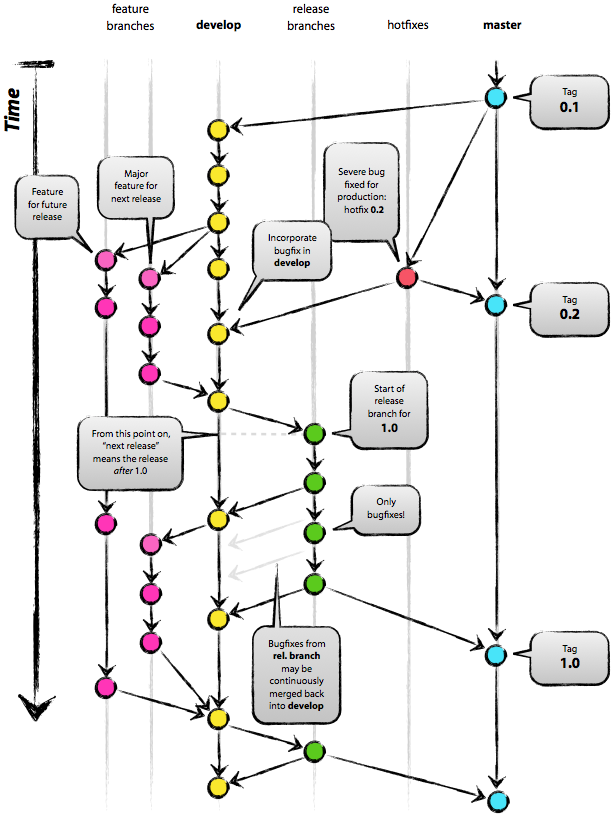
\includegraphics[height=12cm]{images/gitfull.png}
	\caption[Quellcodeverwaltung mit Git]{Git - Feature und Develop Branches}
	\label{fig:git3}
\end{figure}

\subsection{Deployment}
\label{Deployment}

Da die Anwendung auf einem Webserver zur Verf�gung gestellt werden soll, wurde dieser eingerichtet\footnote{http://kallisto.f4.htw-berlin.de}. Daf�r wurde auf den uns zur Verf�gung stehenden Server, als erstes die ben�tigte Software installiert. Um �berhaupt Rails Anwendungen ausf�hren zu k�nnen, wurde Ruby in der Version 1.9.2 und Rails 3.1.1 installiert. Anschlie�end wurde der Apache Webserver installiert. Dieser wurde entsprechend konfiguriert sowie eine PostGreSQL Datenbank installiert. Desweiteren wurde, Capistrano ein OpenSource Deployment-Tool f�r Rails-Anwendungen, installiert. Dabei handelt es sich um eine Software f�r das automatisierte Ausf�hren von Aufgaben auf einem oder mehreren entfernten Servern. Das zentrale Prinzip des Tools ist die vollst�ndige Automatisierung des Verteilungsprozesses. Somit sind die einzelnen Schritte in einem zusammengefasst, wie: Auschecken der Software aus der Versionskontrolle, Ausf�hren der Unit-Tests, �bertragung der Software auf die Ziel-Server, Aktualisierung der Datenbanken und Neustart des Webservers. Diese Schritte w�ren einzeln ausgef�hrt sehr zeitintensiv, fehleranf�llig und zu dem auf Dauer langweilig, vor allem da in einem agilen Entwicklungsprozesses dies relativ h�ufig ausgef�hrt werden muss.


\include{chapter/DatenbasisFunktionalit�t}
\section{File Upload (Paperclip)}
\label{sec:File Upload (Paperclip)}
In der Webanwendung sollen zwei Arten von Datein hochgeladen werden können: Bilder und Audio. Um Dateien zum Server zu laden stehen für Rails zwei Plugins in Rails zur Verfügung Attachment-fu  und Paperclip\footnote{https://github.com/thoughtbot/paperclip}. Wir haben uns für Paperclip entschieden das etwas flexibler als Attachment-fu ist. Möchte man Bilder mit Paperclip zum Server hochladen wird zusätzlich noch das Tool ImageMagick benötigt, welches in der Lage ist verschiedene Versionen eines Bildes zu erstellen sowie die Meta-Informationen auszulesen. Im Model wird definiert welche Art von Datei hochgeladen werden kann. So sollen in für den User als auch für die CD's Bilder hochgeladen werden können. Dazu müssen in der Datenbank zusätzliche Spalten angelegt werden. Paperclip speichert die hochgeladenen Daten nicht in der Datenbank sondern auf dem Dateisystem. In der Datenbank wird lediglich die URL zu der Datei gespeichert. Das macht den ganzen Prozess wesentlich performanter, da die Datenbank nicht so vollgestopft wird. Das hochladen von Audio funktioniert fast genauso, nur das man hier auf andere Mime-Types prüft. Es hat sich gezeigt dsa verschiedene Browser und auch verschiedene Plattformen unterschiedlich mit den Mime-Types umgehen. Mit Paperclip kann sehr schnell ein Datei Upload eingerichtet werden.
\section{MusicBrainz}
\label{sec:MusicBrainz}
MusicBrainz
\section{Tests}
\label{sec:Tests}
Wir haben das Standard Testframework von Rails verwendet um umfangreiche Unit Tests zu schreiben. Dies basiert auf der Idee des Test-Driven-Development. Also zuerst Tests schrieben, schauen wie sie fehlschlagen und dann die Funktionalit�t implementieren und pr�fen ob der Test erfolgreich ist. ie Unit Tests sichern unsere Grundfunktionalit�t. Des weiteren haben wir mit Cucumber Tests geschrieben. Mit Cucumber (Behavior-Driven-Development) ist es m�glich Tests in Prosaform zu schrieben. Das macht die Tests besser lesbarer auch f�r nicht Informatiker. Die Tests werden h�ufig als User Stories geschrieben in der Form: ''Als <Rolle>, m�chte ich <Ziel/Wunsch>, um <Nutzen>''. Umfangreiche Tests wie sie in einem realen Projekt gemacht werden sollten konnten wir aufgrund der beschr�nkten Ressourcen jedoch nicht durchf�hren. Rails eignet jedoch wunderbar f�r ein Test-Driven-Development da es ein Standard Testframwork integriert. 
Hier ist exemplarisch ein Unit Tests f�r das Model User zu sehen. So wird z.B. auf korrekte Form der eMail Adresse getestet und ob die Attribute Name, Vorname, eMail und Passwort gesetzt sind.
\lstinputlisting[language=Ruby]{chapter/test_user.rb}
Hier ist zu sehen wie Tests mit Cucumber geschrieben werden. Zuerst werden sogenannte Features definiert. Diese sind in der <Gegeben> <Eregnis> <Ergebnis> geschrieben. Die feature sind dabei an User Stories angelegt. Diese Art der Tests sind leicht nachzuvollziehen. So k�nnen z.B. auch die Auftrageber eines Projekts welche evtl keine Informatiker sind einbezogen werden.
\lstinputlisting[language=Ruby]{chapter/test_cucumber.rb}
Nat�rlich m�ssen die Features und Szenarien auch automatisiert abgearbeitet werden. dazu findet ein Pattern Matching statt. Trifft eine Regel zu wird der definierte Kurs dieser Regel ausgef�hrt: Hier sind die Regeln und das Pattern Matching zu sehen.
\lstinputlisting[language=Ruby]{chapter/test_pattern.rb}
\chapter{Zusamenfassung}
\label{sec:Zusammenfassung}
In diesem Kapitel fassen die Projektteilnehmer ihre Erfahrungen nach dem Projekt zusammen.
\section{Antonia Ziegler}
Insgesamt würde ich Ruby on Rails als ein sehr modernes und zukunftsorientiertes Framework mit einer grossen Community bezeichnen.
Die Entwicklungsumgebung lässt sich insgesamt gut auf verschiedenen Betriebssystemen aufsetzen. 
Wenn man sich an das gegebene MVC Prinzip hält, ist ein Ruby on Rails Projekt gut erweiterbar und wartbar. 
Was mir am besten gefällt ist die Möglichkeit, oft ziemlich einfach, Plugins einzubinden. Auf Grund der grossen Community gibt es viele Open Source Plugins, welche Funktionen bieten, wie z.B. die Pagenavigation. Diese wiederum sind gut erweiterbar oder anpassbar.
\section{Christian Sandvoss}
Ich finde, das man Railsls sehr gut verwenden kann um auch umfangreiche Webanwendung zu realisieren. Rails stellt ein Grundsystem bereit, das durch viele Pugins erweiterbar ist. Allerdings muss man dabei darauf achten ob das Plugin zur genutzten Rails Version kompatibel ist oder überhaupt noch weiter entwickelt wird. Des weiteren ist bei einigen Plugins die Dokumentation sehr kurz gehalten. Die Dokumentation von Rails ist dagegen, wie ich finde, sehr gut. Es gibt Tutorials zum Einstieg sowie eine aktive Community. Neu für mich war die Arbeit mit JavaScript bzw. JQuery. Es war für mich sehr interessant das Zusammenspiel von verschiedenen Sprachen (Ruby, HTML/CSS, JavaScript) kennenzulernen.

\section{Alexander Miller}
Durch die Realisierung des Projektes konnte ich persönlich feststellen welche Vor- und Nachteile Rails ausweist. Die Verwendung von Rails, können sogar komplexe RIA Web-Anwendungen realisiert werden. Die wesentlichen Prinzipien dieses Frameworks sind Konvention over Configuration und MVC Prinzip. Im Allgemeinen ist Rails sehr gut dokumentiert und hat eine grosse und vor allem aktive Community. Der Umfang an Möglichkeiten ist enorm gross, so dass viele Funktionalitäten problemlos implementiert werden können. Darüber hinaus besteht die Möglichkeit viele Module als Plug-Ins zu integrieren. Der Prozess der Integration von PlugIns ist trivial wenn dieser ausreichend Dokumentiert ist. Leider sind manche PlugIns schlecht dokumentiert, so dass die Auseinandersetzung manchmal viel Zeitaufwand erfordert. Insgesamt bin ich mit dem Framework sehr zufrieden, so dass es nichts dagegen spricht für die Realisierung einer weiteren Web-Applikation Rails zu verwenden.
\section{Christian Bunk}
Ich muss sagen das sich meine Einstellung zu Webframeworks sehr geändert hat. Ich hatte früher nie Lust auf Webentwicklung, da mir Frameworks wie Spring und Struts viel zu kompliziert, zu sperrig, ja sich einfach nicht schön an die Entwicklung von Web Applicationen angefühlt haben. Aber mit Ruby on Rails hat sich das sehr geändert. Schon die Programmiersprache Ruby macht das schreiben von Programmen sehr angenehm. Es ist eine elegante und moderne Sprache. Darauf ein Webframework aufzubauen erscheint nur logisch. Mit Ruby on Rails hat man das Gefühl das alles gut durchdacht ist. Durch das Prinzip Convention over Configuration ist es möglich mit wenig aufwand viel zu erreichen. Alles ist da wo es sein soll und wo es hingehört. Hält man sich an bestimmte Regeln des Frameworks macht die Entwicklugn einfach Spass. Das bedeutet aber nicht das die Entwicklung leicht ist. Im Gegenteil Rails ist ein Framework mit sehr grossem Funktionsumfang. Selbst in den 3 Monaten unserer Entwicklung haben wir in vielen Bereich nur an der Oberfläche gekratzt. Rails bietet eine wunderbare und umfangreiche Dokumentation. Aber um hier hinter alle Konzepte zu steigen braucht es einfach Zeit. Rails bietet mit Erweiterungen durch Module oder Plugins die Möglichkeit Funktionen in seine Webanwendung zu integrieren. Das ist gut solange man nicht mehr Funktionalität braucht als die jeweiligen Plugins bieten. Schwierig wird es wenn man doch eigene oder zusätzliche Funktionen benötigt. Dann muss man versuchen um das Plugin herum zu entwickeln, da meist genaue Dokumentation für die sehr speziellen Fälle fehlen. Mit Rails habe ich auch das Routing, also das mappen von URLs auf bestimmte Methoden in einem Controller, besser verstanden. Das Konzept von Active Record hat mich sehr überzeugt, da hier SChnittstellen und Datenbanken optimal verschmelzen und nicht mehr an jeder Stelle im Code die Datenbank kryptisch ausgelesen oder konfiguriert werden muss. Es wird einfach ein Model definiert, über welches man die Attribute definiert. Diese werden dann automatisch in die Datenbank eingetragen. Rails eignet sich sehr gut für verteilte Entwicklung. Es werden weder Lizenzen benötigt, noch wird dem Programmierer eine IDE aufgezwungen. Alles kann in einem einfachen Texteditor entwickelt werden. Mehr als einen Browser und ein Terminal braucht man dann nicht. Entgegen manchen Vorstellungen das Rails einfach sei muss ich wiedersprechen. MAn braucht viel Zeit um die Konzepte sich zu eigen zu machen. Auch braucht man (wie bei jedem anderen Framework) Zeit um Funktionalitäten zu programmieren. Ich denke eh nicht das man Frameworks nach leichter und schwerer Kategorisieren kann. Ich denke das ich mit Rails wertvolle Erfahrungen gesammelt habe die mir im meinem späteren Berufsleben nützlich sein werden. Ich denke auch das ich mit Rails noch öfter in Zukunft in berührung kommen werde. Rails muss man einfach erlebt haben.
% Literaturverzeichnis:
%\bibliography{C:/literatur}

%Anh�nge:
\appendix

\chapter{Anhang}
\label{sec:Anhang}

\section{Aufgabenstellung}
\label{lst:Aufgabenstellung}


\includepdf[scale=0.88, pages=-, pagecommand={\thispagestyle{headings}}]{pdfs/aufgabe.pdf}

%% Selbst�ndigkeitserkl�rung:
\chapter*{Selbst�ndigkeitserkl�rung}
\label{sec:Selbstaendigkeitserklaerung}
%\addcontentsline{toc}{chapter}{Selbst\"andigkeitserkl\"arung}
\subsection*{Erkl�rung}
\vspace{3ex}
Ich erkl�re, dass ich die vorliegende Seminararbeit selbst�ndig und nur unter Verwendung der angegebenen Quellen und Hilfsmittel angefertigt habe.

\vspace{6ex}
\begin{tabular}{llr}
 \hspace{4cm} & \hspace{1cm} Berlin, den &  \hspace{4cm} \\ \cline{1-1} \cline{3-3}
\end{tabular}


%--------------------------------------
%   Dokumentenende
%--------------------------------------
\end{document}